\documentclass[aspectratio=169,12pt]{beamer}

% ─── Theme & colors ───────────────────────────────────────────────────────────
\usetheme{Madrid}
\usecolortheme{default}

\definecolor{vinotinto}{HTML}{8D191D}
\definecolor{vinotintodark}{HTML}{6B1215}
\definecolor{grisusco}{HTML}{4E6470}
\definecolor{ocre}{HTML}{D8CEA3}
\definecolor{softblue}{HTML}{D6E4F0}
\definecolor{softgreen}{HTML}{D5F5E3}

\setbeamercolor{palette primary}{bg=vinotinto, fg=white}
\setbeamercolor{palette secondary}{bg=vinotintodark, fg=white}
\setbeamercolor{palette tertiary}{bg=grisusco, fg=white}
\setbeamercolor{palette quaternary}{bg=vinotintodark, fg=white}
\setbeamercolor{structure}{fg=vinotinto}
\setbeamercolor{section in toc}{fg=vinotinto}
\setbeamercolor{title}{fg=white}
\setbeamercolor{frametitle}{fg=white, bg=vinotinto}
\setbeamercolor{block title}{bg=vinotinto, fg=white}
\setbeamercolor{block body}{bg=ocre!30}
\setbeamercolor{alerted text}{fg=vinotinto}

\setbeamertemplate{navigation symbols}{}
\setbeamertemplate{footline}{
  \leavevmode
  \hbox{
    \begin{beamercolorbox}[wd=.33\paperwidth,ht=2.25ex,dp=1ex,center]{palette secondary}
      \usebeamerfont{author in head/foot}\insertshortauthor
    \end{beamercolorbox}
    \begin{beamercolorbox}[wd=.34\paperwidth,ht=2.25ex,dp=1ex,center]{palette tertiary}
      \usebeamerfont{title in head/foot}\insertshorttitle
    \end{beamercolorbox}
    \begin{beamercolorbox}[wd=.33\paperwidth,ht=2.25ex,dp=1ex,right]{palette primary}
      \usebeamerfont{date in head/foot}\insertframenumber{} / \inserttotalframenumber\hspace*{2ex}
    \end{beamercolorbox}
  }
}

% ─── Packages ─────────────────────────────────────────────────────────────────
\usepackage[utf8]{inputenc}
\usepackage[T1]{fontenc}
\usepackage[english]{babel}
\usepackage{booktabs}
\usepackage{tikz}
\usepackage{pgfplots}
\pgfplotsset{compat=1.18}
\usetikzlibrary{shapes,arrows.meta,positioning,fit,backgrounds}
\usepackage{xcolor}
\usepackage{array}
\usepackage{fontawesome5}

% ─── Metadata ─────────────────────────────────────────────────────────────────
\title[SIPAM-USCO]{SIPAM-USCO}
\subtitle{AI-Powered Academic Internships \& Tutoring System}
\author[BEINSOF52]{Software Engineering · BEINSOF52 Artificial Intelligence}
\institute[USCO]{Universidad Surcolombiana}
\date{May 2026}

% ─────────────────────────────────────────────────────────────────────────────
\begin{document}

% ── Title slide ───────────────────────────────────────────────────────────────
\begin{frame}[plain]
  \begin{tikzpicture}[remember picture, overlay]
    \fill[vinotinto] (current page.north west) rectangle
      ([yshift=-3.2cm]current page.north east);
    \fill[grisusco] (current page.south west) rectangle
      ([yshift=0.9cm]current page.south east);
  \end{tikzpicture}
  \vspace{0.6cm}
  \centering
  {\color{white}\Huge\bfseries SIPAM-USCO}\\[0.3cm]
  {\color{ocre}\large AI-Powered Academic Internships \& Tutoring System}\\[0.5cm]
  {\color{white}\normalsize Artificial Intelligence Course — BEINSOF52}\\[0.2cm]
  {\color{white}\small Universidad Surcolombiana · Faculty of Engineering · May 2026}
\end{frame}

% ── Outline ───────────────────────────────────────────────────────────────────
\begin{frame}{Agenda}
  \tableofcontents
\end{frame}

% ══════════════════════════════════════════════════════════════════════════════
\section{Introduction \& Problem}
% ══════════════════════════════════════════════════════════════════════════════

\begin{frame}{What is SIPAM-USCO?}
  \begin{columns}[T]
    \begin{column}{0.55\textwidth}
      \textbf{SIPAM} = Academic Internships \& Tutoring Information System
      \vspace{0.4cm}

      Manages \textbf{two core processes} at USCO:
      \begin{itemize}
        \item \alert{Academic Tutoring (Monitorías)} — recruitment, selection, hour tracking
        \item \alert{Field Practices} — multi-stage approval workflow, budget, transport costs
      \end{itemize}
      \vspace{0.4cm}

      \textbf{New:} AI microservice that predicts \\whether a student will be selected as monitor
    \end{column}
    \begin{column}{0.42\textwidth}
      \begin{block}{Tech Stack}
        \footnotesize
        \begin{tabular}{ll}
          \textbf{Backend}   & FastAPI · SQLAlchemy \\
          \textbf{AI}        & Flask · TensorFlow \\
          \textbf{DB}        & PostgreSQL \\
          \textbf{Frontend}  & React 19 · TypeScript \\
          \textbf{Charts}    & Recharts \\
          \textbf{Deploy}    & Netlify · Railway \\
        \end{tabular}
      \end{block}
    \end{column}
  \end{columns}
\end{frame}

\begin{frame}{Problem Statement}
  \begin{alertblock}{Before SIPAM}
    All processes managed via \textbf{paper forms, email and WhatsApp}
  \end{alertblock}
  \vspace{0.3cm}
  \begin{columns}[T]
    \begin{column}{0.48\textwidth}
      \begin{block}{Process Problems}
        \begin{itemize}
          \item No traceability of approvals
          \item Manual monitor selection $\Rightarrow$ inconsistencies
          \item Paper forms take hours to fill
          \item No budget visibility
        \end{itemize}
      \end{block}
    \end{column}
    \begin{column}{0.48\textwidth}
      \begin{block}{Compliance Risk}
        \begin{itemize}
          \item \textbf{Acuerdo 003/2012} — field practice rules
          \item \textbf{Acuerdo 012/2023} — tutoring rules
          \item Min. 30-day advance notice
          \item 66\% consent quorum threshold
        \end{itemize}
      \end{block}
    \end{column}
  \end{columns}
\end{frame}

% ══════════════════════════════════════════════════════════════════════════════
\section{System Architecture}
% ══════════════════════════════════════════════════════════════════════════════

\begin{frame}{System Architecture}
  \centering
  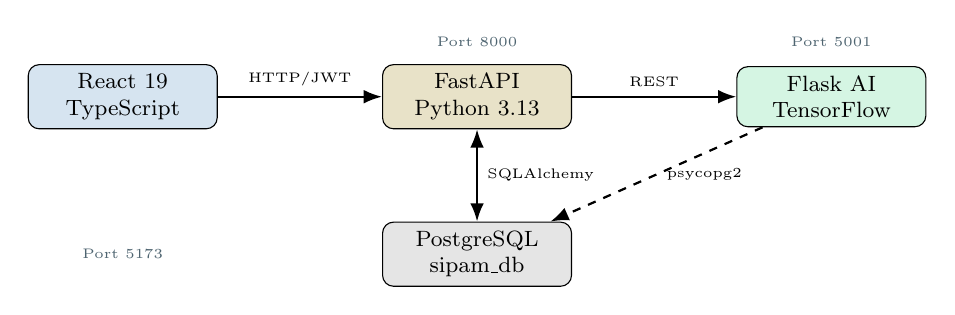
\begin{tikzpicture}[
    box/.style={draw, rounded corners=4pt, minimum width=2.4cm,
                minimum height=0.7cm, align=center, font=\footnotesize},
    user/.style={box, fill=softblue},
    back/.style={box, fill=ocre!60},
    ai/.style={box, fill=softgreen},
    db/.style={box, fill=gray!20},
    arr/.style={->, >=Latex, thick}
  ]
    \node[user]  (react)  at (0,0)    {React 19\\TypeScript};
    \node[back]  (fastapi)at (4.5,0)  {FastAPI\\Python 3.13};
    \node[ai]    (flask)  at (9,0)    {Flask AI\\TensorFlow};
    \node[db]    (pg)     at (4.5,-2) {PostgreSQL\\sipam\_db};

    \draw[arr]           (react) -- node[above,font=\tiny]{HTTP/JWT} (fastapi);
    \draw[arr]           (fastapi) -- node[above,font=\tiny]{REST} (flask);
    \draw[arr,<->]       (fastapi) -- node[right,font=\tiny]{SQLAlchemy} (pg);
    \draw[arr,dashed]    (flask) -- node[right,font=\tiny]{psycopg2} (pg);

    \node[font=\tiny,color=grisusco] at (0,-2)   {Port 5173};
    \node[font=\tiny,color=grisusco] at (4.5,0.7) {Port 8000};
    \node[font=\tiny,color=grisusco] at (9,0.7)   {Port 5001};
  \end{tikzpicture}
  \vspace{0.4cm}
  \begin{columns}[T]
    \begin{column}{0.3\textwidth}
      \centering {\footnotesize\textbf{5 Roles}\\estudiante · profesor\\jefe\_programa · decano · admin}
    \end{column}
    \begin{column}{0.3\textwidth}
      \centering {\footnotesize\textbf{$\approx$75 Endpoints}\\FastAPI + 4 Flask endpoints}
    \end{column}
    \begin{column}{0.3\textwidth}
      \centering {\footnotesize\textbf{26 DB Tables}\\655 users · 51 subjects\\1,262 enrollments}
    \end{column}
  \end{columns}
\end{frame}

\begin{frame}{Key Features Overview}
  \begin{columns}[T]
    \begin{column}{0.48\textwidth}
      \textbf{\color{vinotinto}Tutoring Module}
      \begin{itemize}\footnotesize
        \item Vacancy creation with templates
        \item Application + document upload
        \item Weighted selection RF-MON-05
        \item Voluntary withdrawal (desistir)
        \item Weekly hour tracking (weeks 1–20)
        \item Performance evaluation
        \item PDF forms: FO-14, FO-46
      \end{itemize}
    \end{column}
    \begin{column}{0.48\textwidth}
      \textbf{\color{vinotinto}Field Practices Module}
      \begin{itemize}\footnotesize
        \item 3-stage approval workflow
        \item Digital consent (D-10 window)
        \item Auto-advance at 66\% quorum
        \item INVIAS toll + SICOM fuel costs
        \item Per-diem calculation
        \item PDF forms: FO-05, FO-15, FO-16
        \item Budget tracking
      \end{itemize}
    \end{column}
  \end{columns}
\end{frame}

% ══════════════════════════════════════════════════════════════════════════════
\section{AI Module — Monitor Selection Predictor}
% ══════════════════════════════════════════════════════════════════════════════

\begin{frame}{AI Problem Formulation}
  \begin{block}{Task}
    \textbf{Binary classification} — predict whether a student will be \alert{selected} (1) or
    \alert{not selected} (0) as an academic monitor.
  \end{block}
  \vspace{0.3cm}
  \begin{columns}[T]
    \begin{column}{0.48\textwidth}
      \textbf{Input Features (9)}
      \begin{center}\footnotesize
      \begin{tabular}{ll}
        \toprule
        Feature & Type \\
        \midrule
        promedio & float 0–5 \\
        porcentaje\_creditos & float 0–100 \\
        nota\_asignatura & float 0–5 \\
        nota\_entrevista & float 0–5 \\
        tipo\_monitoria & categorical \\
        semestre\_asignatura & ordinal 1–12 \\
        creditos\_asignatura & ordinal 1–10 \\
        num\_postulantes & integer \\
        num\_monitores\_req. & integer \\
        \bottomrule
      \end{tabular}
      \end{center}
    \end{column}
    \begin{column}{0.48\textwidth}
      \textbf{Target}
      \begin{itemize}
        \item \texttt{seleccionado} $\in \{0, 1\}$
      \end{itemize}
      \vspace{0.4cm}
      \textbf{Data source}
      \begin{itemize}
        \item Real student data from PostgreSQL (655 users, academic profiles)
        \item Synthetic applications generated using RF-MON-05 formula
        \item 200 convocatorias × up to 12 applicants = \textbf{$\sim$1,600 records}
      \end{itemize}
      \vspace{0.2cm}
      \textbf{Labeling formula}
      \[\small\text{puntaje} = n_a \cdot 0.30 + \bar{x} \cdot 0.30 + n_e \cdot 0.40\]
    \end{column}
  \end{columns}
\end{frame}

\begin{frame}{AI Pipeline}
  \centering
  \begin{tikzpicture}[
    box/.style={draw, rounded corners=4pt, minimum width=2.3cm,
                minimum height=0.65cm, align=center, font=\scriptsize},
    proc/.style={box, fill=softblue},
    model/.style={box, fill=softgreen},
    out/.style={box, fill=ocre!60},
    arr/.style={->, >=Latex, thick, color=grisusco}
  ]
    \node[proc]  (db)    at (0,0)      {PostgreSQL\\sipam\_db};
    \node[proc]  (ext)   at (2.8,0)    {extract\_\\dataset.py};
    \node[proc]  (prep)  at (5.6,0)    {prepare\_\\dataset.py};
    \node[proc]  (split) at (8.4,0)    {70/15/15\\+ SMOTE};

    \node[model] (rf)    at (2.1,-1.8) {Random\\Forest};
    \node[model] (xgb)   at (5.6,-1.8) {XGBoost};
    \node[model] (nn)    at (9.1,-1.8) {Neural Net\\(TF)};

    \node[proc]  (eval)  at (5.6,-3.4) {Metrics: Acc · F1 · AUC};
    \node[out]   (best)  at (5.6,-5.0) {Best model (.joblib/.h5)};
    \node[out]   (flask) at (5.6,-6.5) {Flask API — POST /predict};

    \draw[arr] (db) -- (ext);
    \draw[arr] (ext) -- (prep);
    \draw[arr] (prep) -- (split);
    \draw[arr] (split.south) ++(0,0) -- ++(0,-0.5) -| (rf);
    \draw[arr] (split) -- (xgb);
    \draw[arr] (split.south) ++(0,0) -- ++(0,-0.5) -| (nn);
    \draw[arr] (rf) -- (eval);
    \draw[arr] (xgb) -- (eval);
    \draw[arr] (nn) -- (eval);
    \draw[arr] (eval) -- node[right,font=\tiny]{serialize} (best);
    \draw[arr] (best) -- node[right,font=\tiny]{load on startup} (flask);
  \end{tikzpicture}
\end{frame}

\begin{frame}{Three Models Compared}
  \begin{columns}[T]
    \begin{column}{0.32\textwidth}
      \begin{block}{\faTree\ Random Forest}
        \footnotesize
        \begin{itemize}
          \item scikit-learn
          \item n\_estimators: 300
          \item max\_depth: 10
          \item class\_weight: balanced
          \item Tuning: GridSearchCV (3-fold)
        \end{itemize}
      \end{block}
    \end{column}
    \begin{column}{0.32\textwidth}
      \begin{block}{\faBolt\ XGBoost}
        \footnotesize
        \begin{itemize}
          \item xgboost library
          \item n\_estimators: 200
          \item learning\_rate: 0.05
          \item scale\_pos\_weight: auto
          \item Tuning: GridSearchCV (3-fold)
        \end{itemize}
      \end{block}
    \end{column}
    \begin{column}{0.32\textwidth}
      \begin{block}{\faBrain\ Neural Network}
        \footnotesize
        \begin{itemize}
          \item TensorFlow / Keras
          \item Dense(128→64→32→1)
          \item Dropout: 0.3, 0.2
          \item EarlyStopping (patience=10)
          \item ReduceLROnPlateau
        \end{itemize}
      \end{block}
    \end{column}
  \end{columns}
  \vspace{0.4cm}
  \begin{block}{Best Practices Applied}
    \centering\footnotesize
    \begin{tabular}{cccccc}
      70/15/15 split & Stratified & SMOTE & Fixed seed & Serialization & Train $\neq$ Predict \\
      \checkmark & \checkmark & \checkmark & \checkmark & \checkmark & \checkmark \\
    \end{tabular}
  \end{block}
\end{frame}

\begin{frame}{Expected Model Performance}
  \centering
  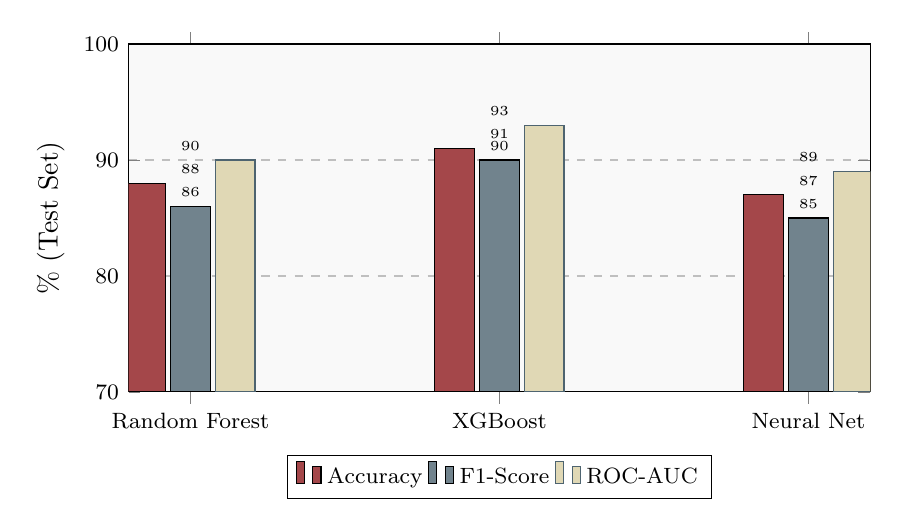
\begin{tikzpicture}
    \begin{axis}[
      ybar,
      bar width=0.5cm,
      width=11cm, height=6cm,
      symbolic x coords={Random Forest, XGBoost, Neural Net},
      xtick=data,
      ymin=70, ymax=100,
      ylabel={\% (Test Set)},
      legend style={at={(0.5,-0.18)}, anchor=north, legend columns=3,
                    font=\footnotesize},
      nodes near coords,
      nodes near coords align={vertical},
      every node near coord/.style={font=\tiny},
      tick label style={font=\footnotesize},
      ymajorgrids=true,
      grid style=dashed,
      axis background/.style={fill=gray!5},
    ]
      \addplot[fill=vinotinto!80]     coordinates {(Random Forest,88) (XGBoost,91) (Neural Net,87)};
      \addplot[fill=grisusco!80]      coordinates {(Random Forest,86) (XGBoost,90) (Neural Net,85)};
      \addplot[fill=ocre!80,draw=grisusco] coordinates {(Random Forest,90) (XGBoost,93) (Neural Net,89)};
      \legend{Accuracy, F1-Score, ROC-AUC}
    \end{axis}
  \end{tikzpicture}
  {\footnotesize\color{grisusco}* Values are illustrative targets; actual results depend on real training data}
\end{frame}

% ══════════════════════════════════════════════════════════════════════════════
\section{Flask AI Microservice}
% ══════════════════════════════════════════════════════════════════════════════

\begin{frame}[fragile]{Flask AI Microservice — Endpoints}
  \textbf{Base URL:} \texttt{http://localhost:5001}
  \vspace{0.3cm}
  \begin{table}
    \footnotesize
    \begin{tabular}{lll}
      \toprule
      \textbf{Method} & \textbf{Endpoint} & \textbf{Description} \\
      \midrule
      GET  & \texttt{/health}                    & Service status \\
      POST & \texttt{/predict}                   & Predict selection outcome \\
      GET  & \texttt{/models/metrics}            & Accuracy, F1, AUC per model \\
      GET  & \texttt{/models/feature-importance} & Feature importances \\
      \bottomrule
    \end{tabular}
  \end{table}
  \vspace{0.3cm}
  \begin{columns}[T]
    \begin{column}{0.48\textwidth}
      \textbf{Request} \texttt{POST /predict}
      \begin{block}{}
        \tiny\ttfamily
        \{\\
        \quad"promedio": 4.1,\\
        \quad"porcentaje\_creditos": 65.0,\\
        \quad"nota\_asignatura": 4.5,\\
        \quad"nota\_entrevista": 4.2,\\
        \quad"tipo\_monitoria": "academica"\\
        \}
      \end{block}
    \end{column}
    \begin{column}{0.48\textwidth}
      \textbf{Response}
      \begin{block}{}
        \tiny\ttfamily
        \{\\
        \quad"selected\_probability": 0.82,\\
        \quad"prediction": "selected",\\
        \quad"confidence": "high",\\
        \quad"model\_used": "XGBoost",\\
        \quad"puntaje\_estimado": 4.23\\
        \}
      \end{block}
    \end{column}
  \end{columns}
\end{frame}

% ══════════════════════════════════════════════════════════════════════════════
\section{Frontend — AI Predictor Widget}
% ══════════════════════════════════════════════════════════════════════════════

\begin{frame}{React AI Predictor Component}
  \begin{columns}[T]
    \begin{column}{0.52\textwidth}
      \textbf{Component:} \texttt{PredictorMonitor.tsx}
      \vspace{0.3cm}
      \begin{itemize}
        \item Input form: GPA, credits, subject grade, interview score, tutoring type
        \item Calls \texttt{POST /api/v1/ia/predecir} (FastAPI proxy)
        \item Shows probability bar (\textcolor{green!60!black}{green} if selected, \textcolor{red!70!black}{red} if not)
        \item Displays estimated score, rank, and selection ratio
        \item \textbf{Model Metrics button} loads comparison chart (Recharts \texttt{BarChart})
        \item Confidence badge: \textit{high} / \textit{medium}
      \end{itemize}
    \end{column}
    \begin{column}{0.45\textwidth}
      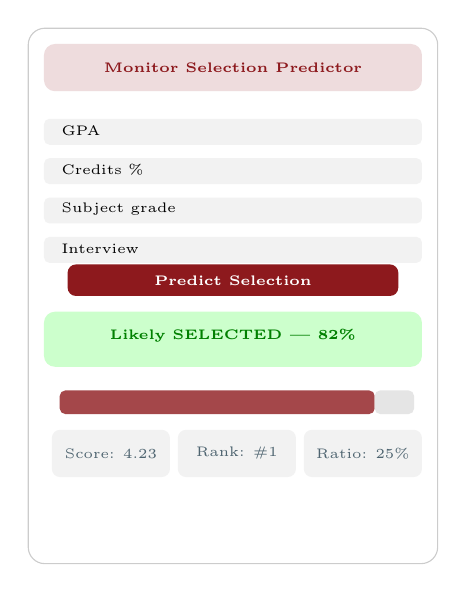
\begin{tikzpicture}
        \draw[rounded corners=6pt, fill=white, draw=gray!40] (0,0) rectangle (5.2,6.8);
        \fill[vinotinto!15, rounded corners=4pt] (0.2,6.0) rectangle (5.0,6.6);
        \node[font=\tiny\bfseries,color=vinotinto] at (2.6,6.3) {Monitor Selection Predictor};

        \foreach \y/\lbl in {5.5/GPA, 5.0/Credits \%, 4.5/Subject grade, 4.0/Interview} {
          \fill[gray!10, rounded corners=2pt] (0.2,\y-0.18) rectangle (5.0,\y+0.15);
          \node[font=\tiny, anchor=west] at (0.3,\y) {\lbl};
        }
        \fill[vinotinto, rounded corners=3pt] (0.5,3.4) rectangle (4.7,3.8);
        \node[font=\tiny\bfseries, color=white] at (2.6,3.6) {Predict Selection};

        \fill[green!20, rounded corners=4pt] (0.2,2.5) rectangle (5.0,3.2);
        \node[font=\tiny\bfseries,color=green!50!black] at (2.6,2.9) {Likely SELECTED — 82\%};

        \fill[vinotinto!80, rounded corners=2pt] (0.4,1.9) rectangle (4.4,2.2);
        \fill[gray!20, rounded corners=2pt] (4.4,1.9) rectangle (4.9,2.2);

        \fill[gray!10, rounded corners=3pt] (0.3,1.1) rectangle (1.8,1.7);
        \fill[gray!10, rounded corners=3pt] (1.9,1.1) rectangle (3.4,1.7);
        \fill[gray!10, rounded corners=3pt] (3.5,1.1) rectangle (5.0,1.7);
        \node[font=\tiny,color=grisusco] at (1.05,1.4) {Score: 4.23};
        \node[font=\tiny,color=grisusco] at (2.65,1.4) {Rank: \#1};
        \node[font=\tiny,color=grisusco] at (4.25,1.4) {Ratio: 25\%};
      \end{tikzpicture}
    \end{column}
  \end{columns}
\end{frame}

% ══════════════════════════════════════════════════════════════════════════════
\section{Cloud Deployment}
% ══════════════════════════════════════════════════════════════════════════════

\begin{frame}{Cloud Deployment Strategy}
  \centering
  \begin{tikzpicture}[
    srv/.style={draw, rounded corners=5pt, minimum width=3cm,
               minimum height=1cm, align=center, font=\footnotesize},
    arr/.style={->, >=Latex, thick, color=grisusco}
  ]
    \node[srv, fill=softblue]   (netlify) at (0,0)    {\faCloud\ \textbf{Netlify}\\\scriptsize React frontend};
    \node[srv, fill=ocre!60]    (railway) at (5,0)    {\faServer\ \textbf{Railway}\\\scriptsize FastAPI backend};
    \node[srv, fill=softgreen]  (flask)   at (10,0)   {\faBrain\ \textbf{Railway}\\\scriptsize Flask AI service};
    \node[srv, fill=gray!20]    (pg)      at (5,-2.2) {\faDatabase\ \textbf{Railway}\\\scriptsize PostgreSQL};

    \draw[arr] (netlify) -- node[above,font=\tiny]{HTTPS} (railway);
    \draw[arr] (railway) -- node[above,font=\tiny]{REST} (flask);
    \draw[arr,<->] (railway) -- node[right,font=\tiny]{TCP 5432} (pg);
    \draw[arr,dashed] (flask) -- ++(0,-1.4) -- node[below,font=\tiny]{read-only} (pg);
  \end{tikzpicture}
  \vspace{0.4cm}
  \begin{columns}[T]
    \begin{column}{0.32\textwidth}
      \begin{block}{Frontend}
        \footnotesize \texttt{netlify.toml}\\
        Build: \texttt{npm run build}\\
        Publish: \texttt{dist/}\\
        SPA redirects: \checkmark
      \end{block}
    \end{column}
    \begin{column}{0.32\textwidth}
      \begin{block}{FastAPI}
        \footnotesize \texttt{Procfile}\\
        \texttt{uvicorn app.main:app}\\
        \texttt{--host 0.0.0.0 --port \$PORT}
      \end{block}
    \end{column}
    \begin{column}{0.32\textwidth}
      \begin{block}{Flask AI}
        \footnotesize \texttt{Procfile} + \texttt{railway.json}\\
        \texttt{python app.py}\\
        Env: \texttt{AI\_PORT=\$PORT}
      \end{block}
    \end{column}
  \end{columns}
\end{frame}

% ══════════════════════════════════════════════════════════════════════════════
\section{Testing}
% ══════════════════════════════════════════════════════════════════════════════

\begin{frame}{Test Coverage}
  \begin{columns}[T]
    \begin{column}{0.48\textwidth}
      \textbf{\color{vinotinto}Unit Tests (pytest-flask)}
      \begin{itemize}\footnotesize
        \item UT-01: Valid input → 200, probability ∈ [0,1]
        \item UT-02: Missing field → 422 with field name
        \item UT-03: promedio > 5 → 422
        \item UT-04: \texttt{/models/metrics} returns 3 models
        \item UT-06: High GPA student → prob ≥ 0.6
        \item UT-07: Minimum eligible student → lower prob
        \item Health check, 404 handler
      \end{itemize}
    \end{column}
    \begin{column}{0.48\textwidth}
      \textbf{\color{vinotinto}Functional \& Integration Tests}
      \begin{itemize}\footnotesize
        \item FT-01: Student sees AI prediction in UI
        \item FT-02: Algorithm selects top-N correctly
        \item FT-03: Full 3-stage practice approval
        \item FT-04: 66\% quorum → auto-advance
        \item IT-01: React → FastAPI → Flask → response within 2s
        \item IT-02: Brute force → 429 on 6th attempt
        \item IT-03: Flask reads student data from DB
      \end{itemize}
    \end{column}
  \end{columns}
  \vspace{0.3cm}
  \begin{block}{Run tests}
    \centering\footnotesize\ttfamily
    pytest ai\_service/tests/test\_predict.py -v
  \end{block}
\end{frame}

% ══════════════════════════════════════════════════════════════════════════════
\section{Results \& Conclusions}
% ══════════════════════════════════════════════════════════════════════════════

\begin{frame}{System Metrics}
  \begin{columns}[T]
    \begin{column}{0.48\textwidth}
      \begin{block}{Database}
        \footnotesize
        \begin{tabular}{lr}
          Users & 655 \\
          Subjects (asignaturas) & 51 \\
          Enrollments & 1,262 \\
          DB tables & 26 \\
          CHECK constraints & 30+ \\
          Indexes & 42 \\
        \end{tabular}
      \end{block}
      \vspace{0.2cm}
      \begin{block}{API}
        \footnotesize
        \begin{tabular}{lr}
          FastAPI endpoints & $\approx$75 \\
          Flask endpoints & 4 \\
          PDF forms generated & 7 \\
        \end{tabular}
      \end{block}
    \end{column}
    \begin{column}{0.48\textwidth}
      \begin{block}{Security}
        \footnotesize
        \begin{itemize}
          \item JWT authentication
          \item Brute-force: 5 attempts/15 min (DB-backed)
          \item Role-based access per endpoint
          \item HTTP security headers (CSP, X-Frame)
          \item MIME type validation on uploads
        \end{itemize}
      \end{block}
      \vspace{0.2cm}
      \begin{block}{AI Compliance}
        \footnotesize
        \begin{itemize}
          \item ✓ 70/15/15 split (reproducible)
          \item ✓ 3 models compared
          \item ✓ SMOTE if imbalanced
          \item ✓ Train script $\neq$ Predict script
        \end{itemize}
      \end{block}
    \end{column}
  \end{columns}
\end{frame}

\begin{frame}{Conclusions}
  \begin{enumerate}
    \item \textbf{Full digitization} of two paper-based institutional processes enforcing both Acuerdo 003/2012 and Acuerdo 012/2023.
    \vspace{0.2cm}
    \item \textbf{Fair and transparent} monitor selection using the official RF-MON-05 weighted formula, now augmented with ML prediction.
    \vspace{0.2cm}
    \item \textbf{AI microservice} (Flask + TensorFlow) cleanly decoupled from the main FastAPI backend following separation-of-concerns best practices.
    \vspace{0.2cm}
    \item \textbf{Production-ready} database with 42 indexes, 30+ CHECK constraints, audit logs, and DB-backed brute-force protection.
    \vspace{0.2cm}
    \item \textbf{Cloud-ready} deployment with Netlify (frontend), Railway (backend + AI) configuration files included.
  \end{enumerate}
\end{frame}

\begin{frame}{Future Work}
  \begin{columns}[T]
    \begin{column}{0.48\textwidth}
      \textbf{Short term}
      \begin{itemize}
        \item Retrain on real postulation data after 2 semesters
        \item Model drift monitoring (Evidently AI)
        \item React Native mobile app for consent signing
      \end{itemize}
      \vspace{0.3cm}
      \textbf{Medium term}
      \begin{itemize}
        \item Integration with USCO academic registry API
        \item Automated PDF generation server-side
        \item WebSocket notifications (real-time)
      \end{itemize}
    \end{column}
    \begin{column}{0.48\textwidth}
      \textbf{Advanced (AI)}
      \begin{itemize}
        \item \textbf{Federated Learning} across faculties (Topic 10)
        \item \textbf{IoT sensors} in greenhouses for practice planning
        \item \textbf{NLP} for automated practice justification review
        \item \textbf{Time series} for budget forecasting
      \end{itemize}
    \end{column}
  \end{columns}
\end{frame}

% ── Final slide ───────────────────────────────────────────────────────────────
\begin{frame}[plain]
  \begin{tikzpicture}[remember picture, overlay]
    \fill[vinotinto] (current page.north west) rectangle
      ([yshift=-4cm]current page.north east);
    \fill[grisusco] (current page.south west) rectangle
      ([yshift=1.2cm]current page.south east);
  \end{tikzpicture}
  \vspace{1.2cm}
  \centering
  {\color{white}\Huge\bfseries Thank you!}\\[0.6cm]
  {\color{ocre}\large Questions?}\\[0.8cm]
  \begin{tabular}{rl}
    {\color{white}\small System:}  & {\color{ocre}\small SIPAM-USCO v1.0} \\
    {\color{white}\small Course:}  & {\color{ocre}\small BEINSOF52 — Artificial Intelligence} \\
    {\color{white}\small Faculty:} & {\color{ocre}\small Engineering — Software Engineering} \\
    {\color{white}\small Date:}    & {\color{ocre}\small May 2026} \\
  \end{tabular}
\end{frame}

\end{document}
